\chapter{Rotor}
Rotoren werden in der Antennentechnik eingesetzt, um die Kommunikation mit nicht-geostationären Satelliten zu ermöglichen, wobei Antennentypen mit hoher Richtwirkung verwendet werden (z.B. Helix-Antenne). In der Regel wird durch diese Methode eine höhere Verstärkung erzielt, als es mit Antennen möglich ist, welche eine größere Abdeckung von Richtungen aufweisen und daher keine Nachführung erfordern. 
\section{Azimut und Elevation}
Die Ausrichtung des Rotors und somit auch der Antenne erfolgt durch die Angabe von zwei Winkeln - Azimut und Elevation - im Gradmaß des astronomischen Horizont-Koordinatensystems \cite{noauthor_astronomische_nodate}. Dabei entspricht das Azimut der auszurichtenden Himmelsrichtung und die Elevation der vertikalen Ausrichtung. Beide Winkelscheitelpunkte werden durch die Position des Rotors definiert. Als Referenzlinie für das Azimut dient die Linie vom Winkelscheitelpunkt nach Norden. Die Referenzlinie für die Elevation bildet der Zenit am Standort des Rotors. Die Elevation entspricht somit dem Komplementärwinkel vom Referenzschenkel zur Linie welche den Winkelscheitel mit dem auszurichtenden Punkt verbindet.

\begin{figure}[H]
	\cite{twcarlson_azimuth_2020}
	\centering
	\includegraphics[width=5.2cm]{../ref/Azimuth-Altitude_schematic_satellit.png}
	\label{fig:Azimut_Elevation_Schematic}
	\caption{Azimut und Elevation Darstellung}
\end{figure}

\section{Yaesu G-5500DC Rotor}
Das Yaesu G-5500DC System \cite{noauthor_yaesu_nodate} besteht aus einem Azimut- und einem Elevation-Rotor sowie dem dazugehörigen Controller und ermöglicht eine gesteuerte Rotation einer unidirektionalen Antenne im Bereich von 0° bis 450° Azimut und 0° bis 180° Elevation.

\subsection{Spezifikationen}
\begin{tabular}{ l l }
	\textbf{Spannungsversorgung:} & 110-120 oder 200-240 VAC \\ 
	\textbf{Motorspannung:} & 22 VDC \\ 
	\textbf{Rotationszeit} (ca.): & Elevation (180°): 65 Sekunden ± 20\% \\
	& Azimut (360°): 60 Sekunden ± 20\% \\
	\textbf{maximaler Dauerbetrieb:} & 3 Minuten \\
	\textbf{Drehmoment:} & Elevation: 12 kgf*m (117.68 Nm)\\
	& Azimut: 6 kgf*m (58.84 Nm)\\
	\textbf{Bremsmoment:} & Elevation: 40 kgf*m (392.27 Nm) \\ &
	Azimut: 40 kgf*m (392.27 Nm) \\
	\textbf{vertikale Belastung:} & 200 kg \\
	\textbf{Ausrichtungsgenauigkeit:} & ± 4\% \\
	\textbf{Windfläche:} & 1 m²\\
	\textbf{Mastdurchmesser:} & 38-63 mm \\
	\textbf{Auslegerdurchmesser:} & 32-43 mm \\
	\textbf{Gewicht} (ca.): & Rotoren: 8 kg \\
	& Controller: 3 kg
\end{tabular}

\subsection{Installation des Rotors}
\subsubsection{Azimut- und Elevationsrotor verbinden}
Um das Yaesu G-5500DC System möglichst Modular anwenden zu können, werden seine Rotoren separat geliefert und müssen für die Anwendung in unserem Fall mithilfe eines mitgelieferten U-Profils wie im Datenblatt beschrieben verbunden werden.

\begin{figure}[H]
	\cite{noauthor_yaesu_nodate}
	\centering
	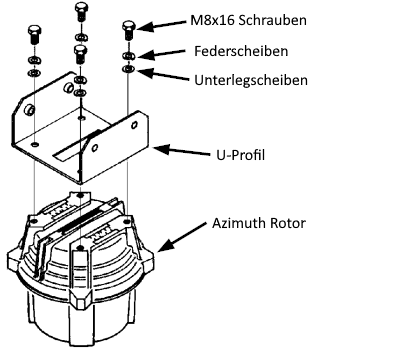
\includegraphics[width=6cm]{../ref/RotorInstallationAzimut.png}
	\label{fig:Rotor_Installation_Azimut_U-Bracket}
	\caption{Azimut Rotor mit U-Profil verbinden}
\end{figure}

\begin{figure}[H]
	\cite{noauthor_yaesu_nodate}
	\centering
	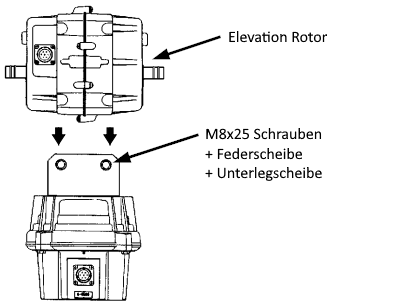
\includegraphics[width=6cm]{../ref/RotorInstallationElevation.png}
	\label{fig:Rotor_Installation_Elevation_U-Bracket+Azimut}
	\caption{Elevation Rotor mit U-Profil und Azimut Rotor verbinden}
\end{figure}



\subsubsection{Kontrollkabel vorbereiten und anschließen}
Für die Ansteuerung der Rotoren werden diese jeweils mit einem 7-Pol-Rundsteckverbinder zum Controller verbunden, wovon 5 Pole verwendet werden. Die Funktion der einzelnen Pins wird im Datenblatt \cite{noauthor_yaesu_nodate} nicht näher beschrieben, konnte allerdings durch Messungen wie folgt bestimmt werden:

Tabelle unbedingt überarbeiten!!!
\newline
\begin{tabular}{| c | l | l |}
	\hline
	\textbf{Pin} & \textbf{Elevation-Funktion} & \textbf{Azimut-Funktion} \\
	\hline
	1 & \multicolumn{2}{| c |}{analoger Ausgang (5V)} \\
	\hline
	2 & \multicolumn{2}{| c |}{analoger Input (0V bis 5V)} \\
	\hline
	3 & \multicolumn{2}{| c |}{analoge Masse} \\
	\hline
	4 & UP Schalter (open collector) & RIGHT Schalter (open collector)\\
	\hline
	5 & DOWN Schalter (open collector) & LEFT Schalter (open collector) \\
	\hline
\end{tabular}

Die Pinbelegung für den 7-Pol-Rundstecker ist im Datenblatt wie folgt angegeben:

\begin{figure}[H]
	\cite{noauthor_yaesu_nodate}
	\centering
	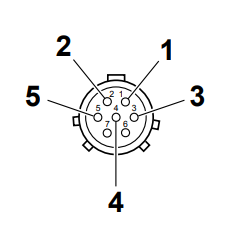
\includegraphics[width=5cm]{../ref/RotorSteckerPinbelegung.png}
	\label{fig:Rotor_Stecker_Pinbelegung}
	\caption{Pinbelegung 7-Pol-Rundstecker (Ansicht vorne)}
\end{figure}

Für die verwendeten Kabel wird im Datenblatt ein Leiterquerschnitt von mindestens 0.5 Quadratmillimeter bei Kabellängen unter 40 Metern und 0.75 Quadratmillimeter bei Kabellängen über 40 Metern vorgeschrieben. Um die Dichtheit der über das Kabel gestülpten Gummikappe zu gewährleisten muss der Außendurchmesser des Kabels zwischen 8.6 bis 10.5 Millimeter betragen.
 
Entsprechend der Pinbelegung im Datenblatt werden die Kabel am anderen Ende mit den Schraubterminal am Rotor Controller verbunden:
\begin{figure}[H]
	\cite{noauthor_yaesu_nodate}
	\centering
	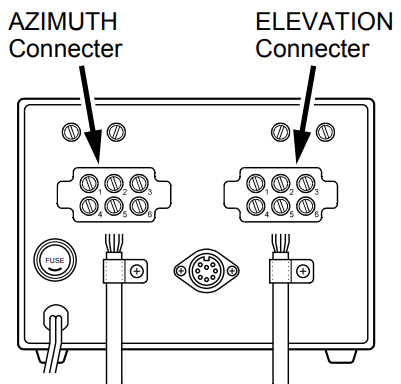
\includegraphics[width=5cm]{../ref/RotorInstallationScrewTerminal.png}
	\label{fig:Rotor_Schraubterminal}
	\caption{Pinbelegung Schraubterminal}
\end{figure}

\subsubsection{Erstinbetriebnahme und kalibrieren der Anzeigen}
Wurden alle Kabel wie beschrieben mit Controller und Rotor verbunden, so kann, nach der Versorgung des Controllers mit Netzspannung, über die DOWN, UP, LEFT und RIGHT Tasten der Rotor manuell bewegt werden. 
\newline
Für die  Nullkalibrierung wird der Controller ausgeschaltet und die Anzeigenadel über die Schraube auf der Vorderseite unter der jeweiligen Anzeige auf den linken Rand ausgerichtet. Für die Anpassung der Vollaussteuerung der Azimut-Anzeige wird der Controller eingeschaltet und der Rotor mithilfe der manuellen Bedientasten bis zum Endschalter nach links gedreht. Die Ausrichtung wird anschließend am Azimut-Rotor, mithilfe von zum Beispiel Klebeband, markiert. Daraufhin wird der Rotor anhand der manuellen Bedientasten nach rechts gedreht, bis er nach einer ganzen Umdrehung wieder den vorher markierten Punkt erreicht. Die Anzeigenadel auf der Azimut-Anzeige sollte sich nun bei 360° befinden, was durch das FULL SCALE ADJ Potentiometer über dem Azimut Schraubterminal auf der Rückseite des Controllers eingestellt werden kann. Für die Kalibrierung des Elevation-Rotor wird dieser mithilfe der manuellen Bedientasten nach oben geschwenkt bis die Ausrichtung genau 180° beträgt. Die Anzeigenadel auf der Elevation-Anzeige sollte sich nun auch bei 180° befinden, was durch das FULL SCALE ADJ Potentiometer über dem Elevation Schraubterminal auf der Rückseite des Controllers eingestellt werden kann.

\subsection {Azimut und Elevation bestimmen}
Die Bestimmung der aktuellen Ausrichtung des Rotors erfolgt über einen von der Rotation des Rotors abhängigen Potentiometer welcher die von Pin 1 zur Verfügung gestellte Spannung teilt. Je nach Ausrichtung ändert sich somit die Spannung am Schleifer des Potentiometers welcher mit Pin 2 verbunden ist. Die Spannung an Pin 2 entspricht somit proportional der Ausrichtung des jeweiligen Rotors. Diese Tatsache wurde durch messtechnische Untersuchungen festgestellt.

\section{Emulation des digitalen Computer Control Interface GS232A/B}
Um den Rotor digital über eine serielle Schnittstelle mit dem Computer steuern zu können, wird das GS232A/B Interface benötigt. Dieses wird über einen 9-Pol DIN-Stecker mit dem G-5500DC Controller verbunden. 
\begin{figure}[H]
	\cite{noauthor_yaesu_nodate}
	\centering
	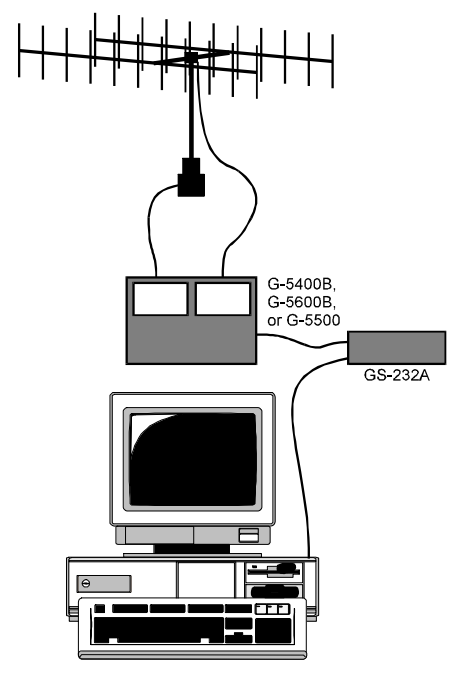
\includegraphics[width=5cm]{../ref/GS232_Prinzipschaltbild.png}
	\label{fig:Rotor_Prinzipschaltbild}
	\caption{Anschlussdiagramm der digitalen Rotorsteuerung}
\end{figure}
Aus finanziellen Gründen wird das GS232A/B mit einem Arduino Uno und entsprechender zusätzlicher Hardware emuliert. Der Preis von € 579,-- für ein GS232B Interface \cite{noauthor_yaesuinterface_nodate} konnte durch den Selbstbau mit Gesamtkosten von € 27,30 um € 551,70 gesenkt werden.

\subsection{Funktionsweise des GS232A/B}
Um das GS232A/B Interface emulieren zu können, bedarf es einer genaueren Betrachtung seiner Funktionsweise und die der beiden Schnittstellen. Diese werden im Datenblatt des Yaesu GS232A/B sowie dem Yaesu G-5500DC \cite{noauthor_yaesu_nodate} erläutert.

\subsubsection{Emulation der seriellen Schnittstelle}
Eine der beiden zu emulierenden Schnittstellen ist die serielle Schnittstelle welche das Interface mit dem Computer verbindet. Basierend auf dem RS232 Protokoll mit einem 8N1 (8 Datenbits ohne Parität und einem Stopbit) Format werden über diese Schnittstelle Befehle für Aktionen oder Messungen vom Computer an das Interface gesendet. Die Baudrate wurde bei der Emulation softwaretechnisch auf 9600 fixiert und kann im Gegensatz zum Original nicht über DIP-Schalter eingestellt werden. Für die Kommunikation verfügt das GS233A/B über einen eigenen Befehlssatz der wie folgt lautet:

\begin{tabular}{| c | l |}
	\hline
	\textbf{Befehl} & \textbf{Funktion} \\
	\hline
	B & Elevation abfragen \\
	\hline
	C & Azimut abfragen \\
	\hline
	C2 & Azimut und Elevation abfragen \\
	\hline
	S & alle Rotationen stoppen \\
	\hline
	A & Azimut Rotation stoppen \\
	\hline
	E & Elevation Rotation stoppen \\
	\hline
	L & Azimut kontinuierlich nach links rotieren (CCW) \\
	\hline
	R & Azimut kontinuierlich nach rechts rotieren (CW) \\
	\hline 
	D & Elevation kontinuierlich nach unten rotieren \\
	\hline 
	U & Elevation kontinuierlich nach oben rotieren \\
	\hline
	Mxxx & zu Azimut rotieren (xxx Azimut in Grad) \\
	\hline
	Wxxx yyy & zu Azimut und Elevation rotieren (xxx = Azimut in Grad, yyy = Elevation in Grad) \\
	\hline
	X1 & Azimut Rotationsgeschwindigkeit 1 (langsam)\\
	\hline
	X2 & Azimut Rotationsgeschwindigkeit 2 \\
	\hline
	X3 & Azimut Rotationsgeschwindigkeit 3 \\
	\hline
	X4 & Azimut Rotationsgeschwindigkeit 4 (schnell)\\
	\hline
	O & Azimut Offset kalibrieren \\
	\hline 
	F & Azimut Vollaussteuerung kalibrieren \\
	\hline
	O2 & Elevation Offset kalibrieren \\
	\hline
	F2 & Elevation Vollaussteuerung kalibrieren \\
	\hline 
	P36 & zu 360 Grad Modus wechseln \\
	\hline 
	P45 & zu 450 Grad Modus wechseln \\
	\hline 
	Z & zwischen Nord- und Südazimut wechseln \\
	\hline
	H & Hilfe \\
	\hline
\end{tabular}

\subsubsection{Emulation der analogen Schnittstelle}
Die Funktionsweise der analogen Schnittstelle, welche über den 8-Pol DIN-Stecker zum G-5500DC Controller verbunden ist, wird im Datenblatt des Rotors \cite{noauthor_yaesu_nodate} wie folgt beschrieben:

\begin{tabular}{| c | l |}
	\hline
	\textbf{Pin} & \textbf{Funktion} \\
	\hline
	1 & liefert 2 bis 4.5 VDC (entspricht 0° bis 180° Elevation) \\
	\hline
	2 & 15.6 VDC mit Pin 8 (Masse) verbinden um nach rechts zu rotieren (CW) \\
	\hline
	3 & 15.6 VDC mit Pin 8 (Masse) verbinden um nach oben zu rotieren \\
	\hline
	4 & 15.6 VDC mit Pin 8 (Masse) verbinden um nach links zu rotieren (CCW) \\
	\hline
	5 & 15.6 VDC mit Pin 8 (Masse) verbinden um nach oben zu rotieren \\
	\hline
	6 & liefert 2 bis 4.5 VDC (entspricht 0° bis 450° Azimut) \\
	\hline
	7 & liefert 8 bis 13.5 VDC mit maximal 100mA \\
	\hline
	8 & Masse \\
	\hline
\end{tabular}

Die Pinbelegung, am Beispiel einer DIN-Buchse, entspricht folgender Grafik: 
\begin{figure}[H]
	\cite{noauthor_yaesu_nodate}
	\centering
	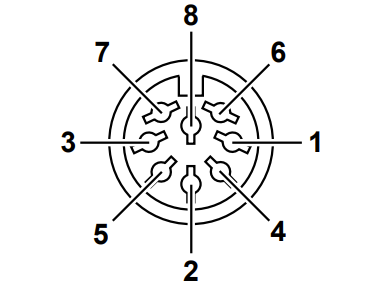
\includegraphics[width=5cm]{../ref/RotorInterfacePinbelegung.png}
	\label{fig:Rotor_Interface_Pinbelegung}
	\caption{Pinbelegung 8-Pol DIN-Buchse (Ansicht vorne)}
\end{figure}

Diese Informationen genügen um nun mithilfe eines Arduino Uno und entsprechendem Shield (zusätzliche Platine die auf den Arduino aufgesetzt wird) das GS232A/B Interface zu emulieren.

\subsection{Software}
Die softwaremäßige Implementierung der Emulation basiert auf dem K3NG Rotator Controller Code \cite{good_k3ngk3ng_rotator_controller_2024} welcher Grundkonstrukte für unterschiedlichste Rotoren und Anwendungen beinhaltet. Diese Software bedient die beiden Schnittstellen und führt diesbezüglich Aktionen entsprechend der vorhergehenden Beschreibung der Funktionsweise des GS232A/B aus. Folgende Konfigurationen und Änderungen wurden an der Software vorgenommen um den benötigten Anforderungen zu entsprechen:

\subsubsection{Änderungen in rotator\_features.h}
In der rotator\_features.h müssen 2 Änderung vorgenommen werden. Die erste Änderung teilt dem Programm mit, dass neben einem Azimut-Rotor auch ein Elevation-Rotor vorhanden ist und dessen Position über eine Spannung am Schleifer eines Potentiometer bestimmt wird. Dazu müssen folgende Präprozessordirektiven dem Programm hinzugefügt werden:

\definecolor{officegreen}{rgb}{0.0, 0.5, 0.0}
\lstset{
	tabsize=3,
	frame=single,
	rulesepcolor=\color{gray},
	xleftmargin=20pt,
	framexleftmargin=15pt,
	keywordstyle=\color{blue}\bf,
	commentstyle=\color{officegreen},
	stringstyle=\color{red},
	numbers=left,
	numberstyle=\tiny,
	numbersep=5pt,
	breaklines=true,
	showstringspaces=false,
	basicstyle=\footnotesize,
	emph={str},emphstyle={\color{magenta}}}
\begin{lstlisting}[language=C++]
#define FEATURE_ELEVATION_CONTROL
#define FEATURE_EL_POSITION_POTENTIOMETER
\end{lstlisting}

Die zweite Änderung deaktiviert die standardmäßig aktivierte Unterstützung für die Verwendung eines Displays. Dazu ist es notwendig folgende Präprozessordirektiven zu löschen oder auszukommentieren.
\begin{lstlisting}[language=C++]
//#define OPTION_DISPLAY_STATUS
//#define OPTION_DISPLAY_HEADING
//#define OPTION_DISPLAY_HEADING_AZ_ONLY
//#define OPTION_DISPLAY_HEADING_EL_ONLY
//#define OPTION_DISPLAY_HHMM_CLOCK
//#define OPTION_DISPLAY_GPS_INDICATOR 
//#define OPTION_DISPLAY_MOON_OR_SUN_OR_SAT_TRACKING_CONDITIONAL
//#define OPTION_DISPLAY_VERSION_ON_STARTUP
\end{lstlisting}

\subsubsection{Änderungen in rotator\_pins.h}
Um das Layout eines Arduino-Shields zu erleichtern werden Pin 8 und Pin 7 wie folgt vertauscht:
\begin{lstlisting}[language=C++]
#define rotate_up 7
#define rotate_ccw 8
\end{lstlisting}

Somit können aus dieser Datei folgende Funktionen für entsprechende Pins des Arduino Uno entnommen werden:

\begin{tabular}{| c | c | l |}
	\hline
	\textbf{Pin} & \textbf{Pin-Mode} & \textbf{Funktion} \\
	\hline
	6 & GPIO-Output & nach rechts Rotieren (Steuersignal für OC-Treiber) \\
	\hline
	7 & GPIO-Output & nach oben Rotieren (Steuersignal für OC-Treiber) \\
	\hline
	8 & GPIO-Output & nach links Rotieren (Steuersignal für OC-Treiber) \\
	\hline
	9 & GPIO-Output & nach unten Rotieren (Steuersignal für OC-Treiber) \\
	\hline
	A0 & ADC (Eingang) & misst die analoge Azimut-Spannung \\
	\hline
	A1 & ADC (Eingang) & misst die analoge Elevation-Spannung \\
	\hline
\end{tabular}

\subsubsection{Änderung in rotator\_settings.h}
In der rotator\_settings.h Datei wird der Azimut Startpunkt auf 0° gesetzt. Das bedeutet der Azimut wird in 0° bis 450° und nicht wie standardmäßig implementiert in -180° bis 360° angegeben.
\begin{lstlisting}[language=C++]
#define AZIMUTH_STARTING_POINT_EEPROM_INITIALIZE 0
\end{lstlisting}

\subsubsection{Änderung in rotator\_debug\_log\_activation.h}
Aufgrund des beschränkten Programmspeicherplatzes auf dem Arduino muss der Debug Dump deaktiviert werden. Dazu ist es notwendig die folgende Präprozessordirektive zu löschen oder auszukommentieren.
\begin{lstlisting}[language=C++]
// #define DEBUG_DUMP
\end{lstlisting}

\subsection{Hardware}
d



